\chapter{State of the art}
\label{cap:estadoDeLaCuestion}

In this chapter, we will explore the fundamental concepts and techniques on which our chess engine is based. This includes board representation, move generation, game trees, etc. Each section will provide an overview of the concepts and techniques used by our engine, and additional tools.

\section{Board representation}
\label{sec:board}

The chessboard is where the game takes place and which serves as the foundation for all operations. In order to store a position setting with its pieces and other additional information like the side to move (the colour that has the turn of movement), the castling rights (the possibilities for each side to castle both short and long, explained in Section~\ref{sec:castling}) or the fifty-move rule counter (explained in Section~\ref{sec:rules} Item~\ref{itm:fifty-move-rule}), we can encounter different types of representations: piece centric, square centric and hybrid solutions. We chose to use bitboards as the primary representation, complemented by a piece list to store the piece on each square (piece centric representation). Additionally, the game state is stored in a bit field.

\paragraph{Bitboard} also known as a bitset or bitmap, is a 64-bit data structure that efficiently represents a chessboard.

\vspace{1em}

\noindent Bitboards can be used to represent different aspects of the board:

\begin{itemize}
    \item All pieces: a bit is set to 1 for every square occupied by a piece, regardless of its type or color.
    \item Pieces by color: a bit is set to 1 for every square occupied by a piece of a specific color. 
    \item Specific piece types: a bit is set to 1 for every square occupied by a specific type of piece.
\end{itemize}

\noindent This structure is highly efficient for operations such as move generation and attack detection, as bitwise operations (e.g., AND, OR, XOR, shifts) can be used to manipulate and query the board state quickly.

\paragraph{Bit field} in constrast to a bitboard, uses a fixed number of bits within an integer to store multiple small values or flags.

\vspace{1em}

\noindent For example, using a 64-bit bitfield, we can allocate 6 bits to store the number of pieces on the board, as $2^6 = 64$ possibilities. This means the bits would occupy an interval from $X$ to $X+5$ inclusive.

\section{Move generation}
\label{sec:move-generation}

An essential part of any chess engine is move generation. It involves generating all possible legal moves from a given position ensuring chess rules.

\vspace{1em}

\noindent There are two types of move generation:

\begin{itemize}
    \item Pseudolegal move generation: generates all moves without considering whether the king is left in check after the move. It requires additional filtering to remove illegal moves which is more computationally expensive than legal move generation.
    \item Legal move generation: generates only moves that are valid according to the chess rules, ensuring that the king is not left in check. The more accurate, the computationally more expensive it is.
\end{itemize}

\noindent We have preferred to use legal move generation because it ensures that the generated moves are correct.

\vspace{1em}

\noindent Additionally, we have chosen to implement \textbf{magic bitboards} for this type of move generator, particularly for sliding pieces such as rooks, bishops, and queens. Magic bitboards use precomputed attack tables and bitwise operations. This approach significantly reduces the computational cost of move generation, enabling the engine to explore deeper levels of the game tree while maintaining accuracy and performance.

\section{Game trees}

Sequential games, such as chess or tic-tac-toe, where players take turns alternately, unlike simultaneous games, can be represented in a game tree or graph. In this representation, the root node is the main position from which we look for the best move, and each subsequent node is a possible option or game state, forming a tree-like structure. This tree has a height or depth that refers to the number of levels or layers in the tree, starting from the root node (the initial game state) and extending to the leaf nodes.

\vspace{1em}

\noindent The depth of a chess game tree is important because it determines the extent to which it will be analysed and evaluated. A depth of 1 represents all possible moves for the current player or side to move, while a depth of 2 includes the opponent's responses to those moves. As the depth increases, the tree grows exponentially, making it computationally expensive to explore all possible states.

\section{Search algorithms}

There are different approaches to find the best move from a position. Some of these search algorithms are: Depth-First Search (DFS), Best-First Search (not to be confused with Breadth-First Search or BFS but they are related) and Parallel Search.

\vspace{1em}

\noindent Note that these search algorithms are the foundation of more advanced and practical algorithms used today. However, explaining them is essential to understand the underlying principles.

\paragraph{Depth-First Search} refers to the process of exploring each branch of a tree or graph to its deepest level before backtracking. Unfortunately, in chess, this cannot be possible because the number of possible moves grows exponentially with the depth of the search tree, leading to the so-called combinatorial explosion. To address this, depth-first search is often combined with techniques like alpha-beta pruning (discussed below) to reduce the number of nodes evaluated, making the search more efficient while still exploring the tree deeply. The following pseudocode illustrates the working of the DFS algorithm:

\begin{lstlisting}[caption={Pseudocode of the Depth-First Search algorithm.}, frame=single, numbers=left, xleftmargin=15pt]
Procedure DepthFirstSearch(Graph G, Node v):
    Mark v as visited
    For each neighbor w of v in G.adjacentEdges(v):
        If w is not visited:
            Recursively call DFS(G, w)
\end{lstlisting}

DFS visits nodes by marking them as visited (line 2) and recursively explores all adjacent nodes until no unvisited nodes remain (lines 3 to 5). It has a worst-case performance of $O(|V| + |E|)$ and worst-case space complexity of $O(|V|)$, with $|V| = \text{number of nodes}$ and $|E| = \text{number of edges}$.

\paragraph{Best-First Search} refers to the way of exploring the most promising nodes first. It is similar to a breadth-first search but prioritizes some nodes before others. They typically require significant memory resources, as they must store a search space (the collection of all potential solutions in search algorithms) that grows exponentially.

\begin{lstlisting}[caption={Pseudocode of the Best-First Search algorithm.}, frame=single, numbers=left, xleftmargin=10pt, breaklines=true]
Procedure BestFirstSearch(Graph G, Node start, Node goal):
    Create an empty priority queue PQ
    Add start to PQ with priority 0
    Mark start as visited

    While PQ is not empty:
        Node current = Remove the node with the highest priority from PQ
        If current is the goal:
            Return the path to the goal

        For each neighbor w of current in G.adjacentEdges(current):
            If w is not visited:
                Calculate priority for w (e.g., using a heuristic)
                Add w to PQ with the calculated priority
                Mark w as visited
\end{lstlisting}

In this case, the priority queue contains nodes along with their associated priorities, which are determined by a heuristic function.

\paragraph{Parallel Search} refers to mulithreaded search, a technique used to accelerate search processes by leveraging multiple processors.

\vspace{1em}

\noindent Next, we will explore some of the most used search algorithms in chess engines.

\clearpage

\subsection{Minimax algorithm}

The \textbf{minimax} algorithm is a decision making algorithm that follows DFS principles. It is based on the assumption that both players play optimally, with one player (the maximizer) trying to maximize his score and the other player (the minimizer) trying to minimize his score. It explores the game tree to evaluate all possible moves and determines the best move for the current player.

\begin{lstlisting}[caption={Pseudocode of the Minimax algorithm.}, frame=single, numbers=left, xleftmargin=15pt, breaklines=true]
Procedure Minimax(Node position, Integer depth, Boolean maximizingPlayer):
    If depth == 0 or position is a terminal node:
        Return the evaluation of the position

    If maximizingPlayer:
        Integer maxEval = -Infinity
        For each child of position:
            Integer eval = Minimax(child, depth - 1, False)
            maxEval = max(maxEval, eval)
        Return maxEval
    Else: // minimizingPlayer
        Integer minEval = +Infinity
        For each child of position:
            Integer eval = Minimax(child, depth - 1, True)
            minEval = min(minEval, eval)
        Return minEval
\end{lstlisting}

\begin{figure}[H]
    \centering
    \begin{tikzpicture}[
        level distance=1.5cm,
        level 1/.style={sibling distance=4cm},
        level 2/.style={sibling distance=2cm},
        circleNode/.style={circle, draw, minimum size=1cm, inner sep=0pt},
        squareNode/.style={rectangle, draw, minimum size=1cm, inner sep=0pt}
    ]
        % Root node
        \node[squareNode] (root) {3}
            child {node[circleNode] (b) {3}
                child {node[squareNode] (d) {3}}
                child {node[squareNode] (e) {5}}
            }
            child {node[circleNode] (c) {2}
                child {node[squareNode] (f) {2}}
                child {node[squareNode] (g) {9}}
            };

        \node[left=1.2cm] at (root) {MAX};
        \node[left=1.2cm] at (b) {MIN};
        \node[left=1.2cm] at (d) {MAX};

        % Edges
        \draw[-{Stealth}, draw=red] (b) -- (root);
        \draw[-] (root) -- (c);
        \draw[-{Stealth}, draw=red] (d) -- (b);
        \draw[-] (b) -- (e);
        \draw[-{Stealth}, draw=red] (f) -- (c);
        \draw[-] (c) -- (g);
    \end{tikzpicture}
    \caption{Example of minimax.}
    \label{fig:minimax}
\end{figure}

\noindent In this example, white is represented by square nodes and black by circle nodes. Note that this example is a binary tree, but there might be more moves or nodes in a real scenario. Each of them wants to maximize or minimize their respective final value in each position. For the leftmost pair of leaf nodes with values of 3 and 5, 3 is chosen because black tries to get the lowest score between them. Then, the other pair of leaf nodes with values of 2 and 9, 2 is chosen for the same reason. Lastly, at the root node, white selects 3 as the maximum number between 3 and 2.

\subsection{Alpha-beta pruning}

Alpha-beta pruning is an optimization of minimax that reduces significantly the number of evaluated nodes in the game tree. It uses two values, alpha and beta, to discard branches that cannot influence the final decision, improving the efficiency.

\begin{lstlisting}[caption={Pseudocode of the Alpha-Beta Pruning algorithm.}, frame=single, numbers=left, xleftmargin=15pt, breaklines=true]
Procedure AlphaBeta(Node position, Integer depth, Integer alpha, Integer beta, Boolean maximizingPlayer):
    If depth == 0 or position is a terminal node:
        Return the evaluation of the position
    If maximizingPlayer:
        Integer maxEval = -Infinity
        For each child of position:
            Integer eval = AlphaBeta(child, depth - 1, alpha, beta, False)
            maxEval = max(maxEval, eval)
            alpha = max(alpha, eval)
            If beta <= alpha:
                Break // Beta cutoff
        Return maxEval
    Else: // minimizingPlayer
        Integer minEval = +Infinity
        For each child of position:
            Integer eval = AlphaBeta(child, depth - 1, alpha, beta, True)
            minEval = min(minEval, eval)
            beta = min(beta, eval)
            If beta <= alpha:
                Break // Alpha cutoff
        Return minEval
\end{lstlisting}

\begin{figure}[H]
    \centering
    \begin{tikzpicture}[
        level distance=1.5cm,
        level 1/.style={sibling distance=4cm},
        level 2/.style={sibling distance=2cm},
        circleNode/.style={circle, draw, minimum size=1cm, inner sep=0pt},
        squareNode/.style={rectangle, draw, minimum size=1cm, inner sep=0pt}
    ]
        % Root node
        \node[squareNode] (root) {3}
            child {node[circleNode] (b) {3}
                child {node[squareNode] (d) {3}}
                child {node[squareNode] (e) {5}}
            }
            child {node[circleNode] (c) {2}
                child {node[squareNode] (f) {2}}
                child {node[squareNode, dashed, red] (g) {X}}
            };

        \node[left=1.2cm] at (root) {MAX};
        \node[left=1.2cm] at (b) {MIN};
        \node[left=1.2cm] at (d) {MAX};

        % Edges
        \draw[-{Stealth}, draw=red] (b) -- (root);
        \draw[-] (root) -- (c);
        \draw[-{Stealth}, draw=red] (d) -- (b);
        \draw[-] (b) -- (e);
        \draw[-{Stealth}, draw=red] (f) -- (c);
        \draw[-] (c) -- (g);
    \end{tikzpicture}
    \caption{Example of alpha-beta pruning.}
    \label{fig:alpha-beta-pruning}
\end{figure}

\noindent In this other example, the red dashed node is pruned because it cannot influence the final decision independently of its value. If its value is less than or equal to 2, it will never improve the previously analyzed value of 3. On the other hand, if its value is greater than 2, black will still choose 2 to minimize the score. Another formal way to explain this is by using $alpha$ and $beta$ values:

\newpage

\begin{figure}[H]
    \centering
    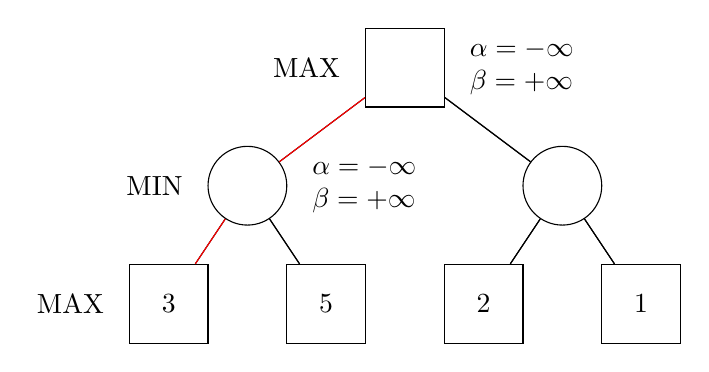
\begin{tikzpicture}[
        level distance=1.5cm,
        level 1/.style={sibling distance=4cm},
        level 2/.style={sibling distance=2cm},
        circleNode/.style={circle, draw, minimum size=1cm, inner sep=0pt},
        squareNode/.style={rectangle, draw, minimum size=1cm, inner sep=0pt}
    ]
        % Root node
        \node[squareNode] (root) {}
            child {node[circleNode] (b) {}
                child {node[squareNode] (d) {3}}
                child {node[squareNode] (e) {5}}
            }
            child {node[circleNode] (c) {}
                child {node[squareNode] (f) {2}}
                child {node[squareNode] (g) {1}}
            };

        % Labels for alpha and beta
        \node[right=0.7cm, align=left] at (root) {$\alpha = -\infty$ \\ $\beta = +\infty$};
        \node[right=0.7cm, align=left] at (b) {$\alpha = -\infty$ \\ $\beta = +\infty$};

        % Node labels
        \node[left=0.7cm] at (root) {MAX};
        \node[left=0.7cm] at (b) {MIN};
        \node[left=0.7cm] at (d) {MAX};

        % Edges
        \draw[-, draw=red] (root) -- (b);
        \draw[-] (root) -- (c);
        \draw[-, draw=red] (b) -- (d);
        \draw[-] (b) -- (e);
        \draw[-] (c) -- (f);
        \draw[-] (c) -- (g);
    \end{tikzpicture}

    \hspace{3em}

    \centering
    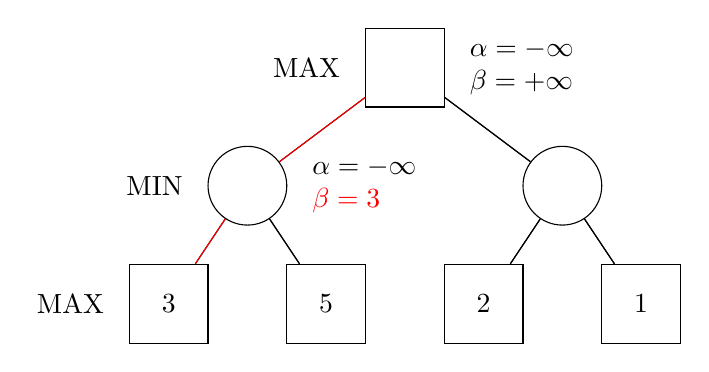
\begin{tikzpicture}[
        level distance=1.5cm,
        level 1/.style={sibling distance=4cm},
        level 2/.style={sibling distance=2cm},
        circleNode/.style={circle, draw, minimum size=1cm, inner sep=0pt},
        squareNode/.style={rectangle, draw, minimum size=1cm, inner sep=0pt}
    ]
        % Root node
        \node[squareNode] (root) {}
            child {node[circleNode] (b) {}
                child {node[squareNode] (d) {3}}
                child {node[squareNode] (e) {5}}
            }
            child {node[circleNode] (c) {}
                child {node[squareNode] (f) {2}}
                child {node[squareNode] (g) {1}}
            };

        % Labels for alpha and beta
        \node[right=0.7cm, align=left] at (root) {$\alpha = -\infty$ \\ $\beta = +\infty$};
        \node[right=0.7cm, align=left] at (b) {$\alpha = -\infty$ \\ $\textcolor{red}{\beta = 3}$};

        % Node labels
        \node[left=0.7cm] at (root) {MAX};
        \node[left=0.7cm] at (b) {MIN};
        \node[left=0.7cm] at (d) {MAX};

        % Edges
        \draw[-, draw=red] (root) -- (b);
        \draw[-] (root) -- (c);
        \draw[-, draw=red] (d) -- (b);
        \draw[-] (b) -- (e);
        \draw[-] (c) -- (f);
        \draw[-] (c) -- (g);
    \end{tikzpicture}

    \hspace{3em}

    \centering
    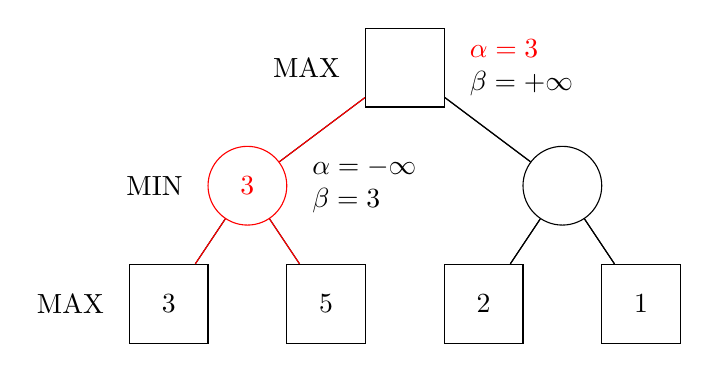
\begin{tikzpicture}[
        level distance=1.5cm,
        level 1/.style={sibling distance=4cm},
        level 2/.style={sibling distance=2cm},
        circleNode/.style={circle, draw, minimum size=1cm, inner sep=0pt},
        squareNode/.style={rectangle, draw, minimum size=1cm, inner sep=0pt}
    ]
        % Root node
        \node[squareNode] (root) {}
            child {node[circleNode, draw=red] (b) {\textcolor{red}{3}}
                child {node[squareNode] (d) {3}}
                child {node[squareNode] (e) {5}}
            }
            child {node[circleNode] (c) {}
                child {node[squareNode] (f) {2}}
                child {node[squareNode] (g) {1}}
            };

        % Labels for alpha and beta
        \node[right=0.7cm, align=left] at (root) {$\textcolor{red}{\alpha = 3}$ \\ $\beta = +\infty$};
        \node[right=0.7cm, align=left] at (b) {$\alpha = -\infty$ \\ $\beta = 3$};

        % Node labels
        \node[left=0.7cm] at (root) {MAX};
        \node[left=0.7cm] at (b) {MIN};
        \node[left=0.7cm] at (d) {MAX};

        % Edges
        \draw[-, draw=red] (root) -- (b);
        \draw[-] (root) -- (c);
        \draw[-, draw=red] (d) -- (b);
        \draw[-, draw=red] (b) -- (e);
        \draw[-] (c) -- (f);
        \draw[-] (c) -- (g);
    \end{tikzpicture}

    \hspace{3em}

    \centering
    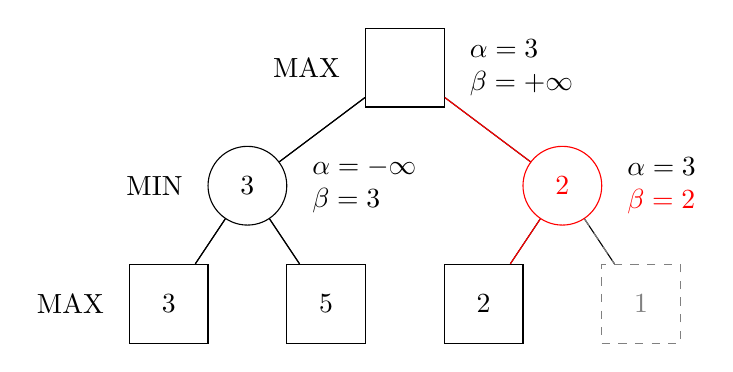
\begin{tikzpicture}[
        level distance=1.5cm,
        level 1/.style={sibling distance=4cm},
        level 2/.style={sibling distance=2cm},
        circleNode/.style={circle, draw, minimum size=1cm, inner sep=0pt},
        squareNode/.style={rectangle, draw, minimum size=1cm, inner sep=0pt}
    ]
        % Root node
        \node[squareNode] (root) {}
            child {node[circleNode] (b) {3}
                child {node[squareNode] (d) {3}}
                child {node[squareNode] (e) {5}}
            }
            child {node[circleNode, draw=red] (c) {\textcolor{red}{2}}
                child {node[squareNode] (f) {2}}
                child {node[squareNode, dashed, gray] (g) {1}}
            };

        % Labels for alpha and beta
        \node[right=0.7cm, align=left] at (root) {$\alpha = 3$ \\ $\beta = +\infty$};
        \node[right=0.7cm, align=left] at (b) {$\alpha = -\infty$ \\ $\beta = 3$};
        \node[right=0.7cm, align=left] at (c) {$\alpha = 3$ \\ $\textcolor{red}{\beta = 2}$};

        % Node labels
        \node[left=0.7cm] at (root) {MAX};
        \node[left=0.7cm] at (b) {MIN};
        \node[left=0.7cm] at (d) {MAX};

        % Edges
        \draw[-] (b) -- (root);
        \draw[-, draw=red] (root) -- (c);
        \draw[-] (d) -- (b);
        \draw[-] (b) -- (e);
        \draw[-, draw=red] (c) -- (f);
        \draw[-, draw=gray, dashed] (c) -- (g);
    \end{tikzpicture}

    \hspace{3em}

    \centering
    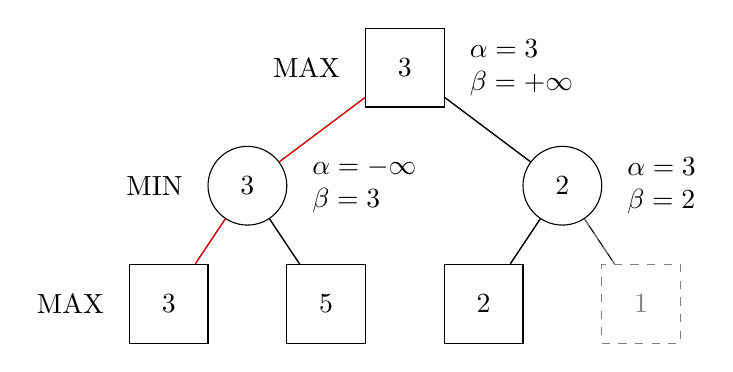
\begin{tikzpicture}[
        level distance=1.5cm,
        level 1/.style={sibling distance=4cm},
        level 2/.style={sibling distance=2cm},
        circleNode/.style={circle, draw, minimum size=1cm, inner sep=0pt},
        squareNode/.style={rectangle, draw, minimum size=1cm, inner sep=0pt}
    ]
        % Root node
        \node[squareNode] (root) {3}
            child {node[circleNode] (b) {3}
                child {node[squareNode] (d) {3}}
                child {node[squareNode] (e) {5}}
            }
            child {node[circleNode] (c) {2}
                child {node[squareNode] (f) {2}}
                child {node[squareNode, dashed, gray] (g) {1}}
            };

        % Labels for alpha and beta
        \node[right=0.7cm, align=left] at (root) {$\alpha = 3$ \\ $\beta = +\infty$};
        \node[right=0.7cm, align=left] at (b) {$\alpha = -\infty$ \\ $\beta = 3$};
        \node[right=0.7cm, align=left] at (c) {$\alpha = 3$ \\ $\beta = 2$};

        % Node labels
        \node[left=0.7cm] at (root) {MAX};
        \node[left=0.7cm] at (b) {MIN};
        \node[left=0.7cm] at (d) {MAX};

        % Edges
        \draw[-, draw=red] (b) -- (root);
        \draw[-] (root) -- (c);
        \draw[-, draw=red] (d) -- (b);
        \draw[-] (b) -- (e);
        \draw[-] (f) -- (c);
        \draw[-, draw=gray, dashed] (c) -- (g);
    \end{tikzpicture}

    \caption{Example of alpha-beta pruning with $\alpha$ and $\beta$ values.}
    \label{fig:alpha-beta-pruning-with-alpha-beta-values}
\end{figure}

\subsubsection{Alpha-Beta Enhancements}

The alpha-beta algorithm has been further improved over time with various enhancements to increase the overall efficiency. Some of these are: transposition tables, iterative deepening, aspiration windows, quiescence search, move ordering\ldots

\vspace{1em}

\noindent Take into consideration that many positions can be reached in different ways. This is formally known as transpositions. Just like in dynamic programming, the evaluations of different positions are stored in a structure, the \textbf{transposition tables}, to avoid repeating the process of searching and evaluating, which improves efficiency. Take the following example:

\vspace{-2em}

\begin{figure}[H]
    \centering
    \begin{minipage}{0.5\textwidth}
        \centering
        \newchessgame
        \chessboard[
            setfen=rnbqkb1r/ppp2ppp/5n2/3p4/3P4/5N2/PPP2PPP/RNBQKB1R w KQkq - 0 1
        ]
    \end{minipage}
    \hspace{1em}
    \begin{minipage}{0.35\textwidth}
        \centering
        French Defense:\\
        1. e4 e6 2. d4 d5 3. exd5 exd5 4. Nf3 Nf6
        \vspace{1em}\\
        Petrov Defense:\\
        1. e4 e5 2. Nf3 Nf6 3. Nxe5 d6 4. Nf3 Nxe4 5. d3 Nf6 6. d4 d5
    \end{minipage}
    \caption{Example of transposition.}
    \label{fig:example-transposition}
\end{figure}

\noindent Both games reach to the same position, although they involve a different number of moves.

\vspace{1em}

\noindent In order to store these different positions and access them in a map or dictionary structure, there is a need for a unique and efficient way to index positions: \textbf{Zobrist hashing}. Zobrist hashing maps a large number of possible positions to a fixed-size hash value, which can lead to collisions, as different positions may produce the same hash. To handle these collisions, storing additional information like the depth is used to verify the correctness of the entry. In some cases, overwriting the older or less relevant entries can be also useful.

\vspace{1em}

\noindent As it is mentioned in \url{https://www.chessprogramming.org/Search}, \textit{<<Depth-first algorithms are generally embedded inside an iterative deepening framework for time control and move ordering issues.>>}. \textbf{Iterative deepening} refers to the combination of DFS with limited depth searches. It performs successive searches by increasing the depth limit at each iteration, allowing you to obtain partial results quickly and improve accuracy over time.

\vspace{1em}

\noindent An important concept related to iterative deepening is the use of \textbf{aspiration windows}. Their main objective is to reduce the search space by narrowing the search bounds. In other words, by adjusting $alpha$ and $beta$ values in each iteration of the iterative deepening. If the value of the evaluation in the iteration falls outside this range or window, a re-search is performed with a wider window to ensure accuracy.

\vspace{1em}

\noindent Another critical concept is \textbf{quiescence search}. This is a search technique used to address the horizon effect at the end of the search. Simply stopping the search at a fixed or desired depth and evaluating the position can lead to inaccuracies, as critical tactical moves, such as captures, are often overlooked.

\begin{quotation}
    \textit{Consider the situation where the last move you consider is QxP. If you stop there and evaluate, you might think that you have won a pawn. But what if you were to search one move deeper and find that the next move is PxQ? You didn't win a pawn, you actually lost a queen. Hence the need to make sure that you are evaluating only quiescent (quiet) positions.}\footnote{\url{https://www.chessprogramming.org/Quiescence_Search}}
\end{quotation}

\vspace{1em}

\noindent Finally, alpha-beta algorithm could not perform well without \textbf{move ordering}. It is important to ensure that best moves are searched first and to reduce the search space of the game tree. Some of the techniques for move ordering are: Most Valuable victim - Least Valuable Aggressor (MVV-LVA) for captures and killer moves for non-captures. 

\paragraph{MVV-LVA} is a heuristic that prioritizes capturing moves by evaluating the value of the piece being captured (the victim) and the value of the piece performing the capture (the aggressor). The goal is to maximize the gain while minimizing the risk. The following example reflects this:

\begin{figure}[H]
    \centering
    \begin{minipage}{0.6\textwidth}
        \centering
        \newchessgame
        \chessboard[
            setfen=r2qr1k1/2p2pp1/p2p1n1p/npb1p2b/3PP3/2P2N1P/PPB2PP1/R1BQRNK1 b Qq - 0 1
        ]
    \end{minipage}
    \caption{Example of MVV-LVA.}
    \label{fig:example-mvv-lva}
\end{figure}

\noindent In this position, it is black's turn to play after white has moved $d4$, black has the option to capture the pawn on $d4$ with the pawn on $e5$ or with the bishop on $c5$. Between the two capturing movements, the best option is to take $d4$'s pawn with $e5$'s pawn because the pawn has less value than the bishop. Then, after $exd4$, white can re-capture with the pawn on $c3$ or the knight on $f3$. If black had taken the pawn with the bishop, white would have won a bishop for a pawn. This simple heuristic that orders what is best in capturing movements for each side can efficiently evaluate tactical exchanges and focus on moves that are more likely to yield a favorable outcome.

\paragraph{Killer moves} is a heuristic that considers moves that produced cutoffs or pruning while searching. When the engine encounters a similar position at the same depth later in the search, it will prioritize the last move that caused a cutoff, potentially leading to faster pruning.

\paragraph{Young Brothers Wait Concept} is a parallel search algorithm designed to optimize the distribution of work among multiple threads. This is particularly effective in alpha-beta pruning, where the search tree is explored selectively. It is divided into two phases: the principal variation move and the wait concept. The principal variation is searched sequentially by the main thread which ensures that the most promising move is evaluated first. Then, once the first move is evaluated, the remaining moves are distributed among multiple threads for parallel evaluation.

\begin{figure}[H]
    \centering
    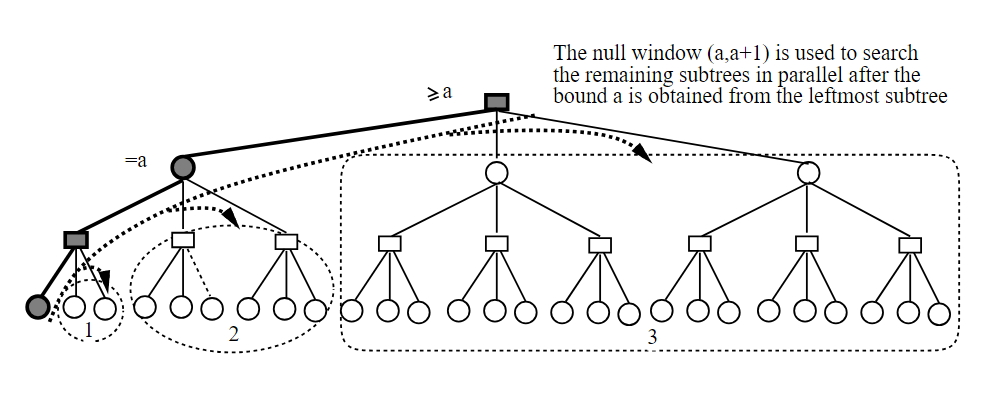
\includegraphics[width=0.8\textwidth]{Imagenes/Bitmap/pvsplitting.png}
    \caption{Principal variation splitting.~\cite{PVSplitting}}
    \label{fig:pv-splitting}
\end{figure}

\section{Evaluation}
\label{sec:evaluation}

For each position, a numerical value is assigned representing how favorable the position is for one side: positive (+) for white and negative (-) for black. These symmetric values were first formulated by~\cite{Shannon1950} and which guide the engine in selecting the best moves during the search process. Generally, this value is expressed in centipawns (cp) that represents one hundredth of a pawn's value. There are two ways to implement it:

\begin{itemize}
    \item Traditional hand-crafted evaluation
    \item Multi-layer neuronal networks
\end{itemize}

\noindent The use of neural networks is beyond the scope of the project, so traditional evaluation has been implemented and discussed below.

\vspace{1em}

\noindent When teaching new chess players how to evaluate their position, assigning a simple value to each piece on board is an effective approach.

\begin{table}[H]
    \centering
    \begin{tabular}{|c|c|}
        \hline
        Piece & Value \\ \hline
        Pawn & 100 \\ \hline
        Knight & 320 \\ \hline
        Bishop & 330 \\ \hline
        Rook & 500 \\ \hline
        Queen & 950 \\ \hline
        King & $\infty$ \\ \hline
    \end{tabular}
    \caption{Standard values assigned to chess pieces in centipawns.}
    \label{tab:piece-values}
\end{table}

\noindent Over the time, there have been different point values for each piece. A table can be found in \url{https://www.chessprogramming.org/Point_Value} in \textit{Basic values} section.

\vspace{1em}

\noindent By summing up the piece values for each side, we end up the concept of material. For example, if white has 1 knight and 1 bishop, while black has 2 bishops, the material calculation is as follows:

\begin{equation}
    (+)(1 \times \mathrm{knightValue} + 1 \times \mathrm{bishopValue}) - (2 \times \mathrm{bishopValue})
\end{equation}
    
\noindent Substituting the standard piece values in centipawns (cp):
    
\begin{equation}
    (1 \times 320 + 1 \times 330) - (2 \times 330) = -10 \, \mathrm{cp}
\end{equation}

\noindent This result indicates that black has a slight material advantage of 10 centipawns.

\vspace{1em}

\noindent There are other material considerations like \textit{bonus for the bishop pair} depending on the position that can be advantageous to control squares of different color, or insufficient material, which refers to situations where neither side has enough pieces to deliver checkmate. This is also mentioned in Section~\ref{sec:rules}.

\vspace{1em}

\noindent However, the higher the level one aims to reach in chess, the greater the need to evaluate other aspects. For instance, there are squares in which the pieces have less value because of their activity.

\begin{figure}[H]
    \centering
    \newchessgame
    \chessboard[
        setpieces={Nh8,Nd4},
        showmover=false,
        pgfstyle=straightmove, color=blue,
        markmoves={h8-g6,h8-f7,d4-b5,d4-b3,d4-c2,d4-c6,d4-e6,d4-e2,d4-f5,d4-f3},
        arrow=to
    ]
    \caption{Knight's movement on corner square and center square.}
    \label{fig:knight-movement-corner-and-center}
\end{figure}

\noindent A knight on a corner has only 2 moves, while one in the center can reach up to 8.

\vspace{1em}

\noindent A way to add this to the evaluation is to have precomputed piece-square tables like the following one for the bishop:

\begin{figure}[H]
    \centering
    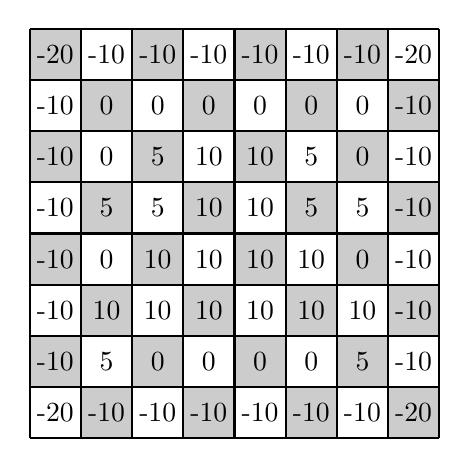
\begin{tikzpicture}[scale=0.65]
        % Draw the chessboard
        \foreach \x in {0,1,...,7} {
            \foreach \y in {0,1,...,7} {
                \pgfmathparse{mod(\x+\y,2) ? "black!20" : "white"}
                \edef\col{\pgfmathresult}
                \fill[\col] (\x,\y) rectangle (\x+1,\y+1);
            }
        }

        % Add the values to the squares
        \node at (0.5,7.5) {-20}; \node at (1.5,7.5) {-10}; \node at (2.5,7.5) {-10}; \node at (3.5,7.5) {-10};
        \node at (4.5,7.5) {-10}; \node at (5.5,7.5) {-10}; \node at (6.5,7.5) {-10}; \node at (7.5,7.5) {-20};

        \node at (0.5,6.5) {-10}; \node at (1.5,6.5) {0}; \node at (2.5,6.5) {0}; \node at (3.5,6.5) {0};
        \node at (4.5,6.5) {0}; \node at (5.5,6.5) {0}; \node at (6.5,6.5) {0}; \node at (7.5,6.5) {-10};

        \node at (0.5,5.5) {-10}; \node at (1.5,5.5) {0}; \node at (2.5,5.5) {5}; \node at (3.5,5.5) {10};
        \node at (4.5,5.5) {10}; \node at (5.5,5.5) {5}; \node at (6.5,5.5) {0}; \node at (7.5,5.5) {-10};

        \node at (0.5,4.5) {-10}; \node at (1.5,4.5) {5}; \node at (2.5,4.5) {5}; \node at (3.5,4.5) {10};
        \node at (4.5,4.5) {10}; \node at (5.5,4.5) {5}; \node at (6.5,4.5) {5}; \node at (7.5,4.5) {-10};

        \node at (0.5,3.5) {-10}; \node at (1.5,3.5) {0}; \node at (2.5,3.5) {10}; \node at (3.5,3.5) {10};
        \node at (4.5,3.5) {10}; \node at (5.5,3.5) {10}; \node at (6.5,3.5) {0}; \node at (7.5,3.5) {-10};

        \node at (0.5,2.5) {-10}; \node at (1.5,2.5) {10}; \node at (2.5,2.5) {10}; \node at (3.5,2.5) {10};
        \node at (4.5,2.5) {10}; \node at (5.5,2.5) {10}; \node at (6.5,2.5) {10}; \node at (7.5,2.5) {-10};

        \node at (0.5,1.5) {-10}; \node at (1.5,1.5) {5}; \node at (2.5,1.5) {0}; \node at (3.5,1.5) {0};
        \node at (4.5,1.5) {0}; \node at (5.5,1.5) {0}; \node at (6.5,1.5) {5}; \node at (7.5,1.5) {-10};

        \node at (0.5,0.5) {-20}; \node at (1.5,0.5) {-10}; \node at (2.5,0.5) {-10}; \node at (3.5,0.5) {-10};
        \node at (4.5,0.5) {-10}; \node at (5.5,0.5) {-10}; \node at (6.5,0.5) {-10}; \node at (7.5,0.5) {-20};

        % Draw the grid
        \draw[thick] (0,0) grid (8,8);
    \end{tikzpicture}
    \caption{Chessboard with precomputed piece-square values for the bishop.}
    \label{fig:piece-square-values-bishop}
\end{figure}

\noindent It is important to consider the game phase to select these piece-square tables, especially in the endgame phase. These phases are:

\begin{itemize}
    \item Opening: where players develop their minor pieces (knights and bishops), control the center of the board and try to ensure king safety.
    \item Middlegame: where players try to create tactical opportunities and attack the opponent's position once they have developed their pieces and secured their king.
    \item Endgame: where players have fewer pieces on the board and the focus is on promoting pawns and achieving checkmate.
\end{itemize}

\noindent In the endgame phase, when there are no queens, king activity becomes extremely significant in supporting the advancement of the pawns.

\vspace{1em}

\noindent In relation to the above and Section \ref{sec:move-generation}, the mobility score measures the number of legal moves a piece can make from its current position. As it is mentioned in \url{https://www.chessprogramming.org/Mobility},
\begin{quotation}
\textit{\dots the more choices you have at your disposal, the stronger your position.}
\end{quotation} This score is calculated as the number of legal moves adjusted for certain factors like blocked moves by friendly pieces (pieces of the same color as the current piece) and enemy attacks (the squares controlled by the opponent).

\vspace{1em}

\noindent During opening and middlegame, king safety is an important factor to consider. When the king has castled, it is crucial to maintain the pawns nearby to shield it from attacks. Generally, it is preferable to keep the pawns unmoved or advanced by only one square. This is called king's shield and a bonus is awarded for each pawn that still has not moved from the castling area.

\vspace{1em}

\noindent On the contrary, king safety penalization can also mean to punish the player based on the number and type of enemy attacks targeting the area around the king.

\vspace{1em}

\noindent All these ensures that positions with exposed kings are evaluated as less favorable. If there are open (no pawns of either color) or semi-open (no pawns of one color but at least one pawn of the opposite color) files near the king, the position is penalized further, as these files provide attacking opportunities for enemy rooks and queens.

\section{How can we determine the strength of our engine?}

This can be answered by playing against other engines and analyzing the results. The most common way to do this is by using the Computer Chess Rating Lists which ranks chess engines based on their performance in various tournaments and matches. By the time being, we have chosen to compare different versions of the engine with Stockfish, currently ranked as the number one on the list. Continue reading to learn about the used tools and read about the work behind it in Section~\ref{sec:tools}.

\subsection{Profiler}

TODO: explain

\subsection{CustomTkinter: Python UI-library}

TODO: explain

\subsection{Cutechess}

TODO: explain

\subsection{Stockfish}

TODO: explain

\subsection{GitHub Actions and workflows}

TODO: explain